\begin{apendicesenv}

\partapendices

\chapter{Cronograma}
\label{schedule_appendix}

\begin{figure}[!htbp]
  \centering
  \includegraphics[width=\textwidth]{figuras/cronogramapc1.eps}
  \caption{Cronograma de Atividades do Ponto de Controle 1. Fonte: autores.}
  \label{fig:cron_d1}
\end{figure}

\begin{figure}[!htbp]
  \centering
  \includegraphics[width=\textwidth]{figuras/cronogramapc2.eps}
  \caption{Cronograma de Atividades do Ponto de Controle 2. Fonte: autores.}
  \label{fig:cron_d1}
\end{figure}

\begin{figure}[!htbp]
  \centering
  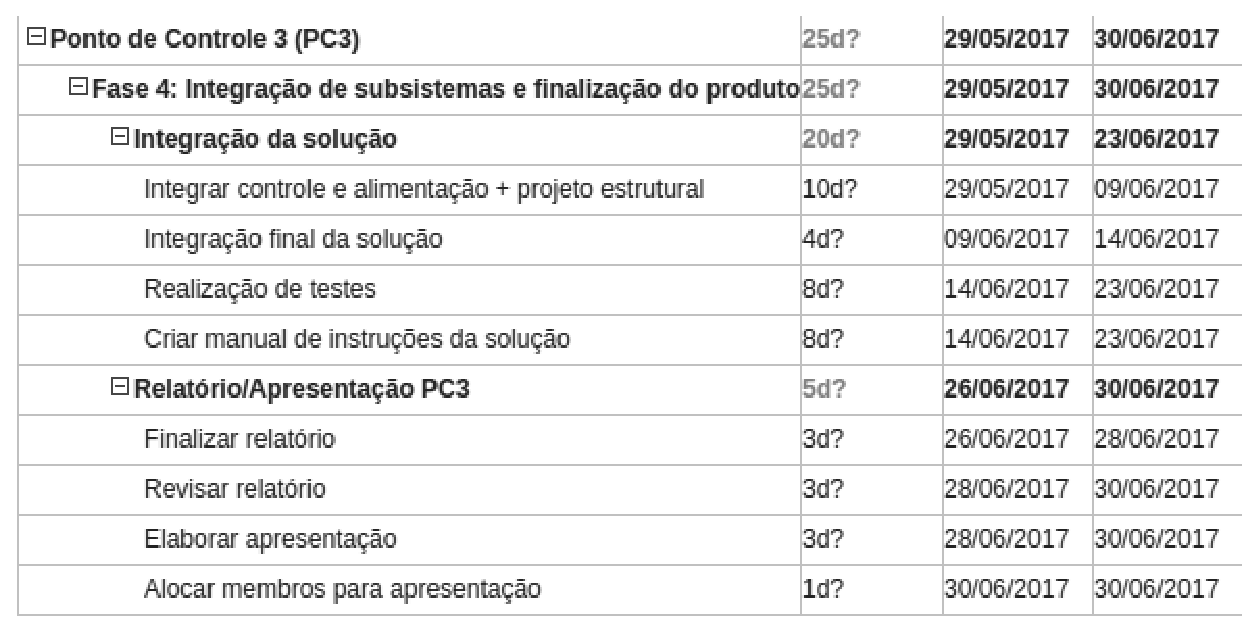
\includegraphics[width=\textwidth]{figuras/cronogramapc3.eps}
  \caption{Cronograma de Atividades do Ponto de Controle 3. Fonte: autores.}
  \label{fig:cron_d1}
\end{figure}

\chapter{Tarefas}
\label{app:tarefas}

Na tabela \ref{tab:atividades1} estão as atividades do subsistema de Processamento de Sinais e Monitoramento;
na tabela \ref{tab:atividades2} estão as atividades do subsistema de Projeto Estrutural;
na tabela \ref{tab:atividades3} estão as atividades do subsistema de Controle e Alimentação.

\begin{table}[h]
  \begin{center}
  \caption{Tarefas realizadas durante o PC1 pelo subsistema PSM.}
  \label{tab:atividades1}
  \begin{tabular}{|l|l|l|l|}
  \hline
  \textbf{Membro} & \textbf{Atividade} & \textbf{Data} \\ \hline\hline
  Gustavo & Criar o cronograma & 24/03 \\ \hline
   & Elicitação de requisitos & 25/03 \\ \hline
   & Definição da arquitetura PSM & 25/03 \\ \hline
   & Finalizar seção do tempo & 28/03 \\ \hline
   & Subseção de tarefas & 31/03\\ \hline
  Wilton & Levantamento de requisitos & 25/03 \\ \hline
  & Gerenciamento dos Custos & 25/03 \\ \hline
   & Definição da arquitetura PSM & 25/03 \\ \hline
  Dylan Guedes & Definição da arquitetura do PSM & 29/03\\ \hline
   & Revisão do Relatório & 31/03 \\ \hline
  Tiago & Definição da arquitetura geral & 25/03 \\ \hline
   & Revisão da metodologia & 26/03 \\ \hline
   & Construção do TAP & 27/03 \\ \hline
  Afonso & Definição arquitetura de PSM & 26/03 \\ \hline
   & Escrita de capítulo de introdução e problemática & 27/03 \\ \hline
   & Definição dos meios de comunicação & 27/03 \\ \hline
   & Definição de requisitos do projeto & 26/03 \\ \hline
  \end{tabular}
  \end{center}
\end{table}

\begin{table}[h]
  \begin{center}
  \caption{Tarefas realizadas durante o PC1 pelo subsistema PE.}
  \label{tab:atividades2}
  \begin{tabular}{|l|l|l|l|}
  \hline
  \textbf{Membro} & \textbf{Atividade} & \textbf{Data} \\ \hline\hline
  Lucas & Definição da arquitetura PE & 25/03 \\ \hline
   & Revisar metodologia & 26/03 \\ \hline
   & Revisar recursos humanos & 27/03 \\ \hline
  Rafael Amado  & Levantamento de requisitos  & 26/03 \\ \hline
   & Elaboração do TAP & 26/03 \\ \hline
   & Mapeamento de peças estruturais & 26/03 \\ \hline
   & Levantamento de riscos & 26/03 \\ \hline
  Nivaldo Lopo  & Busca de possiveis materiais no galpão & 27/03 \\ \hline
   & Revisão dos niveis dos riscos da estrutura & 27/03 \\ \hline
   & Elaboração do EAP & 27/03 \\ \hline
  \end{tabular}
  \end{center}
\end{table}

\begin{table}[h]
  \begin{center}
  \label{tab:atividades3}
  \caption{Tarefas realizadas durante o PC1 pelo subsistema CeA.}
  \begin{tabular}{|l|l|l|l|}
  \hline
  \textbf{Membro} & \textbf{Atividade} & \textbf{Data} \\ \hline\hline
  Cesar Júnior & Elaboração texto arquitetura  & 27/03 \\ \hline
   & Definição dos requisitos de projeto & 28/03 \\ \hline
  Lunara Martins & Pesquisas sobre alimentação da cadeira & 23/03 \\ \hline
   & Elaboração dos riscos do projeto & 27/03 \\ \hline
   & Revisão de requisitos de CeA & 28/03 \\ \hline
   & Revisão do dimensionamento do motor & 29/03 \\ \hline
  Felipe Costa & Definição de arquitetura CeA & 28/03 \\ \hline
   & Levantamento e classificação dos riscos & 29/03 \\ \hline
  Johnson Andrade & Definição arquitetura de Controle & 28/03 \\ \hline
   & Elaboração do texto de arquitetura  & 28/03 \\ \hline
   & Levantamento e classificação de riscos  & 29/03 \\ \hline
  Mariana Andrade & Texto de alocação de recursos humanos & 27/03 \\ \hline
   & Elaboração de requisitos para CeA & 30/03 \\ \hline
   & Dimensionamento do motor & 30/03 \\ \hline
   & Revisão de riscos do projeto & 29/03 \\ \hline
  \end{tabular}
  \end{center}
\end{table}

\end{apendicesenv}
